\chapter{Design and implementation}\label{DesignAndImplementation}
\ifpdf
    \graphicspath{{Chapter3/Chapter3Figs/PNG/}{Chapter3/Chapter3Figs/PDF/}{Chapter3/Chapter3Figs/}}
\else
    \graphicspath{{Chapter3/Chapter3Figs/EPS/}{Chapter3/Chapter3Figs/}}
\fi

The aim of this chapter is to give a thorough description of our concrete implementation of the theoretical framework introduced
in Chapter \ref{TheoreticalFramework}. We list and provide an explanation of the individual
components and also explain our reasoning for certain design choices. In section \ref{WebApp} we present a proof-of-concept web application that 
we have developed in order to demonstrate how the different components can be integrated together to form a platform for event detection. 

\section{System Overview}
Figure \ref{SystemOverview} shows an overview of the system architecture which is a pipeline of the individual components we described
in Chapter \ref{TheoreticalFramework}. Each one of these components is depicted as an independent module in the figure.  
Initially, historical tweets from a service provider (Twitter API or another provider) are retrieved and stored in an 
appropriate format in the database. Subsequently, the system receives a stream of tweets from the database and processess and 
transforms them in a format that is appropriate for clustering. The next step in the pipeline is the actual clustering of the tweets 
in order to detect groups of tweets discussing the same topic. Then, the extracted clusters are processed in order to identify the events 
and generate their summaries. Finally, a visual representation of the results should be generated in order to aid understanding of the events.\\

\begin{figure}[htbp]
  \begin{center}
    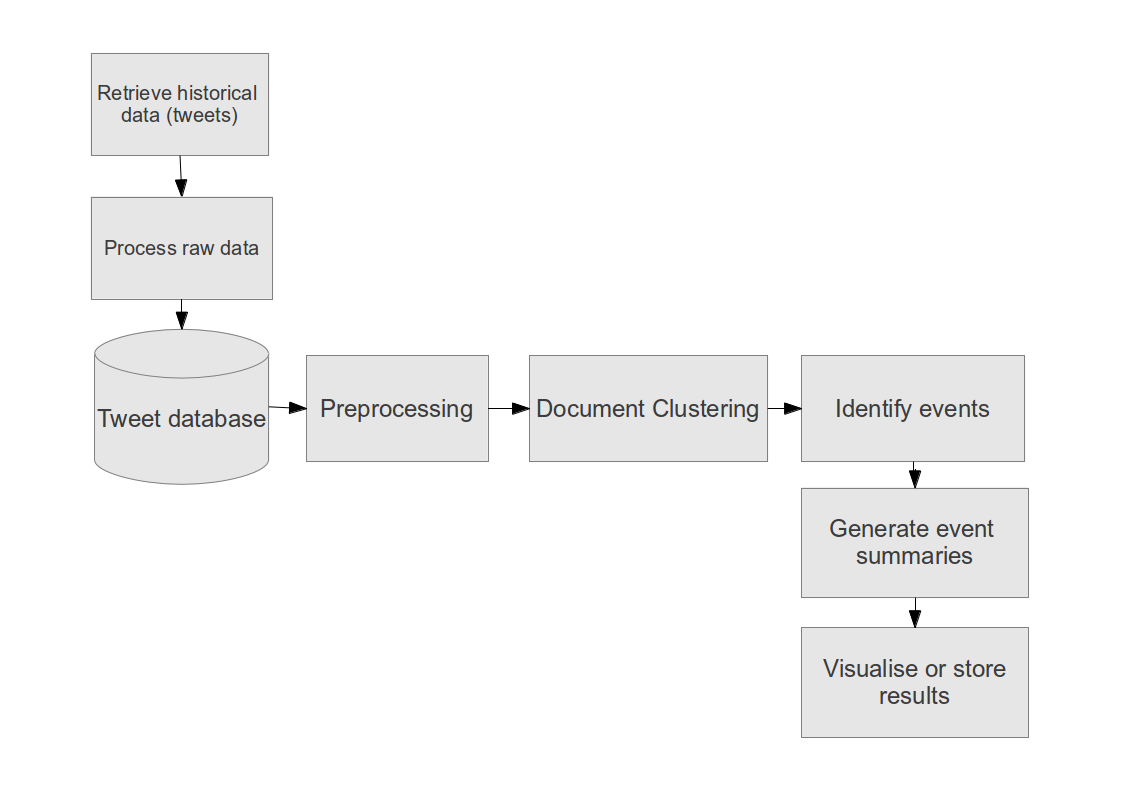
\includegraphics[height=3in, width=6in]{system-overview}
    \caption{System overview - The event extraction system comprises of several independent components.}
    \label{SystemOverview}
  \end{center}
\end{figure}

\subsection{Tools}
In the process of implementing the system we have mainly used our implementation of the algorithms but several third-party 
software libraries were used to implement the sub-components of the system. Here we describe the main tools we have used.\\ 

\begin{itemize}
 \item \textbf{Python:} 
 \item \textbf{Natural Language Toolkit (NLTK) :} 
 \item \textbf{Lucene:} 
 \item \textbf{Orange:} 
\end{itemize}\vspace{15pt}

\section{Data Retrieval}
A vital part of our system is the retrieval of a large amount of historical tweets. The first obvious choice is the Twitter API which provides tweets, user profiles and several metadata related to Twitter. They also provide a streaming API which is commonly used to collect tweets in real time. However, the main problem with the Twitter API is that it has a very restrictive limit policy (150 requests per hour) and it does not provide access to tweets posted more than a few days ago. This is a problem for our project since we require access to historical data. The solution is to use other archiving services and there are numerous possibilities. However, it is essential for us to have direct access to their database through an API and unfortunatelly, most of them do not provide an API. We have found that Topsy \footnote{http://topsy.com/} provides an excellent API \footnote{http://code.google.com/p/otterapi/} and direct access to tweets from 2009 up to the present day. Additionally, Topsy API is free and the limit policy allows us to retrieve our data easily. Therefore, we have decided to use Topsy Otter API with its Python bindings.

\section{Raw text processing}
The raw tweets received from Topsy are not processed and therefore we must apply some pre-processing steps before storing them in the database. The reasons for pre-processing were outlined clearly in Chapter \ref{TheoreticalFramework}. Figure \ref{RawTextProcessingOverview} depicts the sub-components of the raw text pre-processing module.\\

\begin{figure}[htbp]
  \begin{center}
    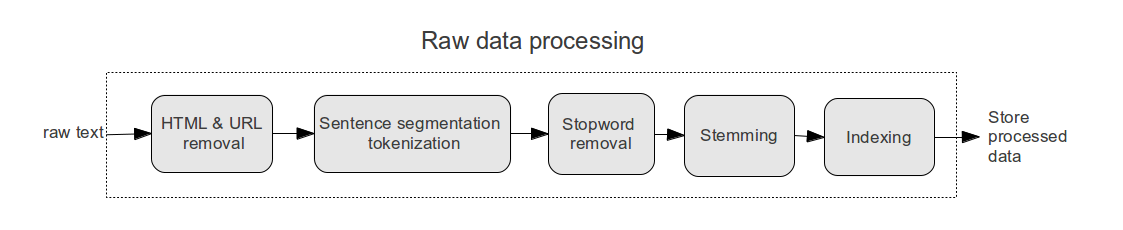
\includegraphics[height=1.5in, width=6in]{raw-data-processing}
    \caption{The raw data processing module - All the steps neccessary to convert raw documents to a format suitable for storage in a database.}
    \label{RawTextProcessingOverview}
  \end{center}
\end{figure} 

\textbf{HTML and URL removal:} Firstly, we need to clean the tweets from the URLs and HTML tags since they are useless for clustering. In order to do so we have used regular expressions which capture any possible format of URLs or HTML code.\\

\textbf{Sentence segmentation and tokenisation:} For the implementation of this module we have used the default sentence segmenter of NLTK and the WordPunctTokenizer to tokenise the resulting sentences. The reason we have used WordPunctTokenizer is due to the fact that it can handle alphabetic and non-alphabetic characters. Since it is common to use non-alphabetic characters in a tweet we could find an easy way to remove characters such as '.' and ','. Consider for example the following tweet:
 
\begin{figure}[htbp]
  \begin{center}
    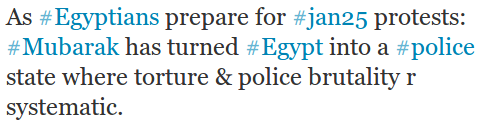
\includegraphics[height=1in, width=4in]{tweet-text}
    \label{TweetText}
  \end{center}
\end{figure}

The output from this module will be a list of words containing the terms \textbf{[ 'as', 'egyptians', 'prepare', 'for' 'jan25', 'protests', 'mumbarak', 'has', 'turned', 'egypt', 'into', 'a', 'police', 'state', 'where', 'torture', 'police', 'brutality', 'r', 'systematic' ]}. Note that characters '.', '\#', '\&' and ':' have been removed. \\

\textbf{Stopword removal:} The next step is to remove common English words that doesn't provide any information. NLTK provides a dictionary of the English stopwords and we have used it to filter out stopwords from the tweets. Using the list of words extracted for the example above the output of the stopword removal module will be: \textbf{['egyptians', 'prepare', 'jan25', 'protests', 'mumbarak', 'turned', 'egypt', 'police', 'state', 'torture', 'police', 'brutality', 'r', 'systematic' ]}

\textbf{Stemming:} Once we have the list of our terms we can use a stemming algorithm to reduce the words to their root. Our implementation uses the widely used Porter stemmer which is also implemented in NLTK. The final list of words after the stemming becomes \textbf{['egyptian', 'prepar', 'jan25', 'protest', 'mumbarak', 'turn', 'egypt', 'polic', 'state', 'tortur', 'polic', 'brutal', 'r', 'systemat' ]}\\

\textbf{Indexing:} Just before storing the tweets in the database we take a last step which is to index the tweets. For each word occuring in our corpus we aggregate all the tweets that contain that term and the position of that word in the document. Effectively, we create a mapping from a word to a list of documents. In our implementation the inverted index is very important since it allows us to construct term-documment vectors easily and filter terms and documents. For example, using our index we can find the words that appear either too often or less frequently and filter them out. This is used to reduce the dimensionality of our dataset by removing unneccesary words. Alternatively, we
can remove documents/tweets which contain keywords that appear too often or less frequently. In our implementation we have used PyLucene which is the Python equivalent of the Lucene indexing library. The library allow us to do what we have discussed above and in addition it provides helper functions such as the calculation of the TF-IDF weigtings for a dataset.
 
\section{Clustering}

So far we have managed to retrieve and store historical tweets in our database. The next module in our pipeline is to perform clustering on the tweets and identify clusters which discuss the same topic. The clustering module (Figure \ref{ClusteringOverview}) is responsible to construct the term-frequency vectors by processing the dataset and subsequently to apply a clustering algorithm on the dataset. 

\begin{figure}[htbp]
  \begin{center}
    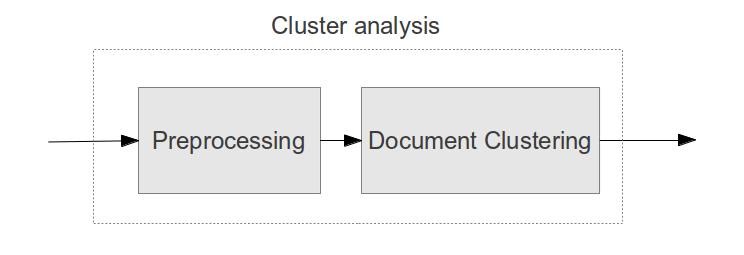
\includegraphics[height=1.5in, width=4in]{clustering-overview}
    \caption{The cluster analysis module - The dataset is processed to construct the term-frequency vectors and then a clustering algorithm is used to identify the clusters.}
    \label{ClusteringOverview}
  \end{center}
\end{figure} 

There are several candidates algorithms for clustering documents and we have decided to implement four of them. The theoretical background of these algorithms is outlined in Chapter \ref{TheoreticalFramework} and in Chapter \ref{Evaluation} we present a thorough comparison of these algorithms with respect to their performance in clustering tweets.  
In the next section we provide our implementation of these algorithms and the components that are needed for clustering. 

\subsection{AbstractClusterer}
The four different algorithms presented in this section are the k-Means, DBSCAN, Non-negative Matrix Factorisation (NMF) and online clusterers. Although these methods are fundamentally different they share some common functionality. For example the pre-processing steps, such as the construction of the term-frequency vectors is identical for all of them. Also, all of the algorithms output the clusters using the same format and therefore the methods for visualising the clusters will be identical. The architecture of the software components responsible for implementing the clustering functionality tries to incorporate this common functionality as well as accomodating the different core implementation of each algorithm. The UML diagram (Figure \ref{UMLClusterers}) below illustrates the different components of the clustering module. The AbstractClusterer class implements all the common functionalities such as add\_document, construct\_term\_freq\_matrix, plot\_scatter and dump\_clusters\_to\_file. Since each algorithm uses a different method to perform the actual clustering task, the AbstractClusterer class do not provide any implementation for the "run" function. This is the responsibility of each derived clusterer. 

\begin{figure}[htbp]
  \begin{center}
    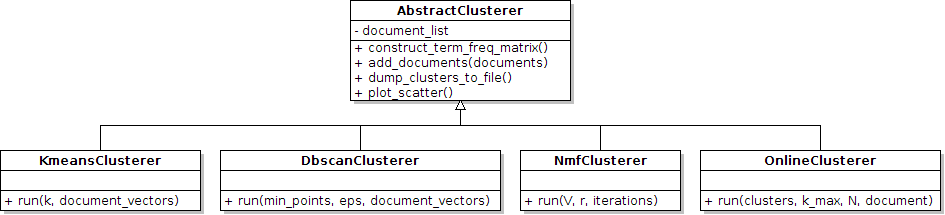
\includegraphics[height=2.0in, width=6in]{clusterers-uml}
    \caption{The four derived clusterers share common functionality which is implemented in the AbstractClusterer class. }
    \label{UMLClusterers}
  \end{center}
\end{figure}    
 
The main functionality of the AbstractClusterer is to construct the term-frequency vector for each document and consequently the term-frequency matrix $a$ which has a row for each document and a column for each distinct term in the dataset. This will convert the corpus in the vector space representation. Listing \ref{AbstractClustererSnippet} shows the pseudocode for implementing the construct\_term\_freq\_matrix function. We retrieve the dataset from the database and we find all the distinct terms that occur across all the documents. Then the term-frequency matrix is initialised and we iterate over the documents filling in the elements of the matrix with the TF-IDF weight of each term. The function returns the matrix $a$.

\begin{lstlisting}[language=Python, label=AbstractClustererSnippet, caption=Pseudocode for constructing the term-frequency matrix for a dataset]
def construct_term_freq_matrix(corpus):
  '''
  Inputs: 
  corpus: The collections of documents we will cluster
  
  Outputs:
  a: A nxm matrix where n is the number of documents 
     in the corpus and m the number of distinct terms
     in the corpus.  
  '''
  terms = find_distinct_terms(corpus)
  a = initialise_term_frequency_matrix(rows=len(corpus), 
                                        columns=len(terms))
  
  for i, document in enumerate(corpus):
    for term in document
      a[i][term] = tf_idf(term, document, corpus)
    
  return a 
\end{lstlisting}

In the next pages we discuss the implementation of the concrete clusterers which implement the second sub-component of the cluster analysis module. We also show some preliminary results of the clustering process.\\

\subsection{k-Means clusterer}
Listing \ref{KmeansClustererSnippet} shows the pseudocode for k-Means clustering algorithm. The algorithm works by randomly initialising k centroids and then finding out which document vectors are closest to the centroid. Then the centroid is recomputed based on the mean of the vectors belonging to this centroid and this mean value becomes the new centroid. An additional check is performed again to ensure that all the vectors are still belonging to that cluster after the recomputation of the centroid. This procedure is repeated until there are previous cluster membership has not changed. Note that the distance() function can be any of the three distance measures described in the previous chapter.

\begin{lstlisting}[language=Python, label=KmeansClustererSnippet, caption=Pseudocode for k-Means algorithm]
def run(k, document_vectors):
  '''
  Inputs: 
  k: the number of clusters
  document_vectots: the set of n document 
                     vectors I={i1,i2,..,in}
  
  Outputs:
  C: cluster centroids {c1, c2, ..., ck}
  m: I --> C the cluster membership
  '''
  C = random_centroid_initialisation()
  
  distances = []
  for vector in document_vectors
    for c in C:
      dist = distance(c, vector)
      distances.append(dist)
    m[vector] = min(distances)

  while has_changed(m):
    for c in C:
      c = recompute_centroid(c, vectors_of(c))   
    
    for vector in document_vectors
      for c in C:
        dist = distance(c, vector)  
        distances.append(dist)
      m[vector] = min(distances)
  return C, m

\end{lstlisting}
\subsection{DBSCAN clusterer}
Listing \ref{DbscanClustererSnippet} shows the pseudocode for the DBSCAN clustering algorithm. Initially,
all documents are marked as unvistied and the cluster list is empty. Then the algorithm randomly selects a new document vector, marks it as visited and finds all its neighbors than are within a distance eps. The set of neighbors is called ε-neighborhood and we denote it here by N. In order to calculate the distance we use one of the three predefined distance measures. If N does not contain at least min\_pts then we mark this vector as a noise point. Otherwise, a new cluster is created which contains this vector and all the objects in N are added to a candidate set. DBSCAN iteratively adds to the new cluster those documents in the N that do not belong to any cluster. For any object in the ε-neighborhood DBSCSAN checks again its own ε-neighborhood N' and if it has at least min\_pts those document vectors are added to the N. This continues, with DBSCAN adding new documents in the new cluster, until N is empty. Finally, to find the next cluster DBSCAN selects a new unvisited document vector and continues the same process until all vectors have been visited.  

\begin{lstlisting}[language=Python, label=DbscanClustererSnippet, caption=Pseudocode for DBSCAN algorithm]
def run(min_points, eps, document_vectors):
  '''
  Inputs: 
  eps: the radius parameter
  min_pts: the neighborhood density threshold.
  document_vectors: the set of n document vectors 
                     I={i1,i2,..,in}
  
  Outputs:
  C: the clusters and the document vectors 
     belonging to them
  '''
  C = [] #The cluster list
  mark_all_vectors_as_unvisited(document_vectors)
  
  while not all_is_visited(document_vectors):  
    vector = pick_random(document_vectors)
    mark_as_visited(vector)
    neighbors = get_neighbors(document_vectors, vector)
    if len(neighbors) >= eps:
      new_cluster = create_cluster(vector) 
      C.append(new_cluster)
      for n_vector in neighbors:
        if not is_visited(n_vector) 
          mark_as_visited(n_vector)
          n_neighbors=get_neighbors(document_vectors,n_vector)
          if len(n_neighbors) >= eps:
            neighbors.append(n_neighbors)
        if not_in_cluster(n_vector):
          new_cluster.add(n_vector)
    else:
      mark_as_noise(vector) 
  return C
\end{lstlisting}
\subsection{Non-negative matrix factorisation (NMF) clusterer} Our implementation is based for NMF is based on the paper [put ref here for Learning the parts of objects by nonnegative matrix factorization]. The method accepts as input the term-frequency matrix $V$ the number of basis vectors to generate $r$ and the number of optimisation iterations. The algorithm starts from non-negative initialisations for W and H and then iteratively updates W and H until a factorisation $V \approx WH$ such that $| V - WH |$ is minimal. If the number of maximum iterations has not been reached and the error did not change since the last iteration then the algorithm halts and return W and H. Listing \ref{NmfClustererSnippet} shows the pseudocode for the NMF algorithm. The notation $A.T$ indicates that we shoud take the transpose of the matrix $A$.
  
\begin{lstlisting}[language=Python, label=NmfClustererSnippet, caption=Pseudocode for the NMF algorithm]
def run(V, r, iterations):
  '''
  Inputs: 
  V: the matrix to factorize
  r: number of basis vectors to generate
  iterations: number of optimisation
             iterations to perform
  
  Outputs:
  W: a set of r basis vectors
  H: represenations of the columns of V in 
     the basis given by W
  '''
  
  C = size(V,1) #dimensionality of examples (# rows)
  N = size(V,2) #number of examples (columns)

  W = rand(N,r);
  H = rand(r,C);
  
  previous_error = 0
  error = 0
  for i in xrange(iterations):

    #Update W
    W2 = dot(dot(W, H), H.T) + 10**-9
    W *= dot(V[:,:], H.T)
    W /= W2
    
    #Update H
    H2 = dot(dot(W.T, W), H) + 10**-9
    H *= dot(W.T, V[:,:])
    H /= H2                                     
    
    previous_error = error
    error = sqrt( sum((V[:,:] - dot(W, H))**2 ))
    
    if i > 1 and error:
      if previous_error == error:
        break
  return W, H
  
\end{lstlisting}

\subsection{Online clusterer}
The rest of the algorithms operate on the dataset as a whole. Since we are interested in clustering a vast amount of documents these approaches are expensive. However, we can use a category of clustering algorithms called sequential or online clustering methods. The main difference is that they cluster each individual example sequentially by updating the clusters once this specific example is presented to the system. Therefore, an online algorithm is scalable. Usually, this kind of algorithms are centroid-based and the mean values of centroids are updated using a moving average. This is the the main difference of an online clusterer and this why they are faster. However, in our case whenever we are presented with a new document the term-frequency vectors of all the previous documents must be updated. This operation is computationally expensive and therefore instead of considering all the previous document one can use sliding window approach. For example if we are presented with the $ith$ document, denoted as $x_i$ and our window size is N then only the documents $\{ x_{i-1}, x_{i-2},..., x_{i-N}\}$ will be used for clustering. This can provide us with an extra performance boost. \\\\
Our implementation is illustrated in pseudocode in Listing \ref{OnlineClustererSnippet} and it can be summarised in three main steps:

\begin{enumerate}
  \item Find the closest centroid and move it closer to the new document vector. 
  \item Merge the two closest centroids, c1 and c2, which means that we are left with a redundant centroid c2.
  \item Set the redundant centroid equal to the document vector. 
\end{enumerate}
These three steps satisfy three important criteria. Firstly, the within-cluster variance is minimised by Step 1 and the between-cluster distance is maximised by Step 2. Finally we capture the changes in the data distribution after a new document is clustered by Step 3 since we are treating each new document as an indication to a potential new cluster.\\\\
In the algorithm there are two cases when we need to update the location and the size of an existing centroid. The first one is when a centroid is the closest to a new document and it must be moved closer to it. The location of the closest centroid, $c$, is updated according to the following update rule location:
\begin{eqnarray}
c_{center} \leftarrow c_{center} + \frac{d_{center} - c_{center}}{c_{size} + 1}    
\end{eqnarray}  
where $c_{center}$ is the centroid's location, $c_{size}$ is the number of documents this centroid represents and $d_{center}$ is the document that we are trying to get closer to. The size of a centroid is increased by one each time a new document is assigned to it. The second case for updating is when two clusters, $c_1$ and $c_2$ need to be merged. The update rules for the location and the size are then defined as:
\begin{eqnarray}
c1_{center} \leftarrow \frac{c1_{center} \times c1_{size} + c2_{center} \times c2_{size}}{c1_{size} + c2_{size}} \\
\end{eqnarray}  
\begin{eqnarray}
c1_{size} \leftarrow c1_{size} + c2_{size} 
\end{eqnarray}  


\begin{lstlisting}[language=Python, label=OnlineClustererSnippet, caption=Pseudocode for the online clustering algorithm]
def run(clusters, k_max, N, document):
  '''
  Inputs:
  N: the size of the document window
  k_max: the maximum number of clusters we can identify 
  document: the new document to be clustered 

  Outputs:
  clusters: returns the updated clusters
  '''    
  #construct a new term-frequency vector based on the new
  #document and consider only the last N documents. 
  vector = construct_term_freq_vector(self.document_list, 
                                      document, 
                                      N)

  distances = []
  for centroid in clusters:
    dist = distance(centroid, vector)
    distances.append(dist)
  
  #find the closest centroid (Step 1)
  closest = min(distances)
  closest.add(vector)

  #update the centroids center  
  closest.size += 1
  closest.center += (vector-closest.center)/closest.size
  
  if len(clusters)>=k_max and len(clusters)>1:
    #merge the most similar clusters (Step 2)
    merged = merge_closest(clusters)
  
  
  #create a new cluster for this document (Step 3)
  newc = Cluster(vector)
  clusters.append(newc)
  return clusters
  
def merge_closest(clusters):
  c1, c2 = find_closest()
  c1.center=(c1.center*c1.size+
            c2.center*c2.size)/(c1.size+c2.size)
  c1.size+=c2.size
  c2.remove() #c2 is now merged with c1 so remove it
  return c1
    
\end{lstlisting}

\subsection{Clustering results}
[TODO: add screenshots from the clustering results]

\section{Identifying events}
[TODO: Complete this section]

\section{Generating automatic summaries}
So far we have managed to retrieve historical tweets from Twitter and identify clusters of topics that were discussed in them. After that we have filtered out the irrelevant clusters and kept the important ones which are considered as the events. Some of these events contain a lot of tweets and therefore it would be extremely tedious for a human observer to understand what happened during that event. Therefore, at this point we must implement our automatic summary generators. The main task here is to find the most important tweets, keywords and named entities. In the next sections we describe how we have implemented the functionality to extract this information. An overview of the summarisation module is shown in Figure \ref{SummarisationOverview}.  

\begin{figure}[!htbp]
  \begin{center}
    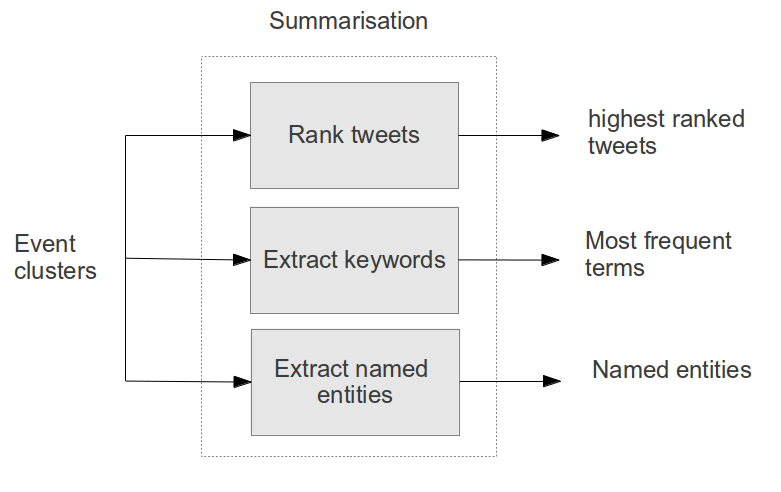
\includegraphics[height=3.0in, width=6in]{summarisation-overview}
    \caption{The summarisation module receives the event clusters and outputs the highest ranked tweetsm keywords and entities in each cluster.}
    \label{SummarisationOverview}
  \end{center}
\end{figure} 

\subsection{Ranking tweets}
The first sub-component of the summarisation module is to device a way to rank the tweets in order to extract the most \emph{relevant}, \emph{useful} and \emph{high-quality} tweets. These are the three criteria that our summarises must meet. We described them in more detail in Chapter \ref{TheoreticalFramework} and in the following sections we will look into how we implemented two algorithms to meet these requirements.  

\subsubsection{Abstract summariser}
Again, the two summarisers share some common functionality and like the clusterers we define an AbstractSummariser which is responsible to provide these common functions. The derived summarisers will inherit these functions and also provide their own concrete implementation of the run (the function which performs the actual ranking) function. Figure \ref{SummariserArchitecture} illustrates the software architecture. 

\begin{figure}[htbp]
  \begin{center}
    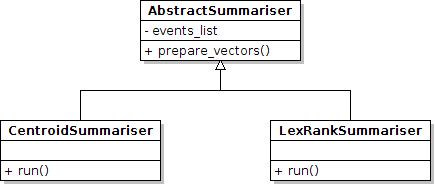
\includegraphics[height=2.0in, width=4in]{summarisers}
    \caption{The two derived summarisers share common functionality which is implemented in the AbstractSummariser class. }
    \label{SummariserArchitecture}
  \end{center}
\end{figure} 

\subsubsection{Centroid-based summariser}
The main idea behind this summariser is that tweets closer to the event's cluster centroid are more likely to be useful and relevant to the event than others which are distant. Also, the third criterion is met since the centroid's weights are calculated based on the average of the tweets' vectors and therefore typos and spelling mistakes are more likely to be ruled out. The implementation of this algorithm is straightforward and is shown in Listing \ref{CentroidSummariserSnippet}. First we retrieve the term-frequency vectors for all the documents in the cluster we want to rank. Then we calculate the centroid by averaging the individual vectors. Finally, the cosine similarity of each document and the centroid is calculated and we return a sorted list of similarities. The similarity acts as a ranking score since the closer a document is to a centroid the highest its ranking.  

\begin{lstlisting}[language=Python, label=CentroidSummariserSnippet, caption=Pseudocode for the centoid-based summariser.]
def run(event_cluster):
  '''
  Inputs:
  event_clusters: The cluster for which we want to rank 
                  the tweets.
  Outputs:
  ranked: A list of ranked tweets in descending order. 
  '''        
  vectors = event_cluster.get_document_vectors()
  
  #Calculates the centroid by averaging the individual
  #vectors of alll the documents in the cluster.
  centroid = calculate_centroid(vectors)
  
  similarities = []
  for vector in vectors:
    sim = cosine(vector, centroid)
    similarities.append(sim)
  
  return sorted(similarities)
  
\end{lstlisting}

\subsubsection{LexRank summariser}
As we have described in Chapter \ref{TheoreticalFramework} 
LexRank is an algorithm where we define a graph that has nodes for the sentences to be summarised the 
edges are placed between two sentences that are similar to each other. We can then rank all the sentences 
based on the expected probability of a random walker visiting each sentence using equation \ref{LexRankEquation}. \\
The main differentiation in our implementation to the usual LexRank algorithm is that we scale the probability of 
jumping to the next node based on the cosine similarity of two nodes. The reason we do this is that we want to favor jumping to 
a node that discuss a more similar topic. We can implement this alteration by scaling the summation in the equation by the cosine similarity 
of the nodes $u$ and $v$. Since the similarity is in the range $[0, 1]$ an identical node it won't be discounted whereas a node with similarity equals 0 
it will be ignored. The equation the becomes:

\begin{eqnarray}\label{LexRankEquationModified}
L(u) = \frac{d}{N} + (1-d) * sim(u, v) \sum_{v \in adj[u]}^{\infty}\frac{L(v)}{deg(v)}
\end{eqnarray} 

\begin{lstlisting}[language=Python, label=CentroidSummariserSnippet, caption=Pseudocode for the centoid-based summariser.]
def run(event_cluster, threshold, tolerance):
  '''
  Inputs:
  event_clusters: The cluster for which we want to rank 
                  the tweets.
  Outputs:
  ranked: A list of ranked tweets in descending order. 
  '''        

  vectors = event_cluster.get_document_vectors()      
  n = len(vectors)
  adjacency_matrix,degree=calculate_similarities(vectors, 
                                              threshold)
  
  for i in xrange(n):
      for j in xrange(n):
        adjacency_matrix[i][j] = adjacency_matrix[i][j] 
                                            / degree[i]
                                            
  ranked = power_method(adjacency_matrix, tolerance)        
  
  return ranked
    
def power_method(self, m, epsilon):
  n = len( m )
  p = [1.0 / n] * n
  while True:
      new_p = [0] * n
      for i in xrange( n ):
          for j in xrange( n ):
              new_p[i] += m[j][i] * p[j]
      total = 0
      for x in xrange( n ):
          total += ( new_p[i] - p[i] ) ** 2
      p = new_p
      if total < epsilon:
          break
  return p  
\end{lstlisting}

\subsection{Named entity and keyword extraction}
The other two parts of the summarisation module is the named entity and keyword extraction. The keyword extraction task is straightforward since we mereley want to 
find the keywords in the event cluster that have the heighest TF-IDF weights. Therefore, it is just a matter of looking up the TF-IDF weighted term-frequnecy vectors and 
find the best keywords. For the name entity extraction task we decided to use the built-in capabilities of NLTK. More specifically, NLTK contains functions which can implement part of speech tagging and then extract named entities based on these tags. The pseudocode for this task is not included since it has not been implemented by us. For example if the input to the system is a tweet with the following content: "Most protesters in Cairo have gathered in front of the maspiro building, protest in Alex is also picking up ‪\#jan25" then the output will be "Cairo, GPE" meaning that Cairo is identified as a location. Named entity extraction is not always accurate and therefore we must be careful when we decide whicj entities to output. For example in the above tweet the system could erroneously identify the word "Alex" as a human name. However, in reality the author of the tweet mentioned the name of the city Alexandria in Egypt. Therefore, in order to minimise the possibility of a misinterpretation we decided to output only the named entities that appear most frequently in the cluster's tweets. 

\section{Classifying users}
In our system user classification is important since it can allows us to understand the events even better. The user distribution in an event can give us insight into what has been discussed and ascribe quality to the events. For example, events that include a large amounts of tweets from journalists or media organisations are more likely to be of high quality with respect to reliability and descriptive quality. \\\\
Since we want to investigate the events that took place during the Arab Spring we know that the important types of users we need to consider are: Media organisations, Journalists, Activists, Celebrities and Common individuals. In order, to classify a user to one of these categories we must know its profile. A user profile is an N-dimensional vector of attributes that are used to discriminate different user types. We have narrowed down these attributes to be:
\begin{itemize}
  \item Retweet ratio
  \item Link ratio
  \item How ofthen this user gets retweeted?
  \item Ratio of replies
  \item Ratio of mentions
  \item Followers to followees ratio 
\end{itemize}
The first attribute is a simple count of the number of retweets of a user divided by the overall number of their tweets. Retweets are most commonly used by common individuals to share a tweet they liked but they are rarely used by media organisations. Therefore, if the retweet ratio is very small we may suspect that this is a media organisation. The second attribute is also an important feature as we can very easily identify a media organisation by the number of tweets that contain links. The reason is because Twitter accounts for media organisation are used to share links of their articles. If a user gets retweeted too often this is usually an indication that they are popular or their tweets are considered interesting. Therefore, the number of times a user gets retweeted can be a measure of its popularity and therefore if we observe a user which gets retweeted frequently we may assume they are a celebrity, a journalist or even an activist. A user can reply to another user by using the "@" character followed by the username and the same holds for when a user wishes to mention another user in a tweet. The difference between a mention and a reply is that replies start with the "@username" pattern whereas in tweets that mention someone this pattern can appear anywhere. Replies are usually used by common people to start and maintain conversations but are very rarely used by celebrities and media organisations. Finally, one of the most discriminating features is the followers to followees ratio. The reason for this is because celebritiesand media organisations have very high followers to followees ratio but common people have very low ratio. Activists and journalists are in the middle of the spectrum.\\\\
The task now becomes to collect a training dataset which contains labelled user profiles. This will be used to train our classifiers. The obvious way to collect the data is by manually looking up users on Twitter and constructing their profiles. However, this will be a tedious and time consuming process and thus we decided to automatically collect our data. We have done that by crawling a website called Twtrland \footnote{http://twtrland.com/} which provides Twitter user statistics.   

\subsection{Crawling user profiles}
A web crawler is a type of software agent that browses websites in a methodical and automated way in order to retrieve up-to-date information. This technique is used in our case to retrieve user profiles from Twtrland. Our web crawlers are constructed using an open source crawling library for Python called Scrapy \footnote{http://scrapy.org/}. A crawler is given the URL of user profile on Twtrland and then it parses the HTML code of that page and automatically retrieves the information we need. A typical page on Twtrland is shown in Figure \ref{TwtrlandPage} and the rectangles indicate the information we collect. 

\begin{figure}[htbp]
  \begin{center}
    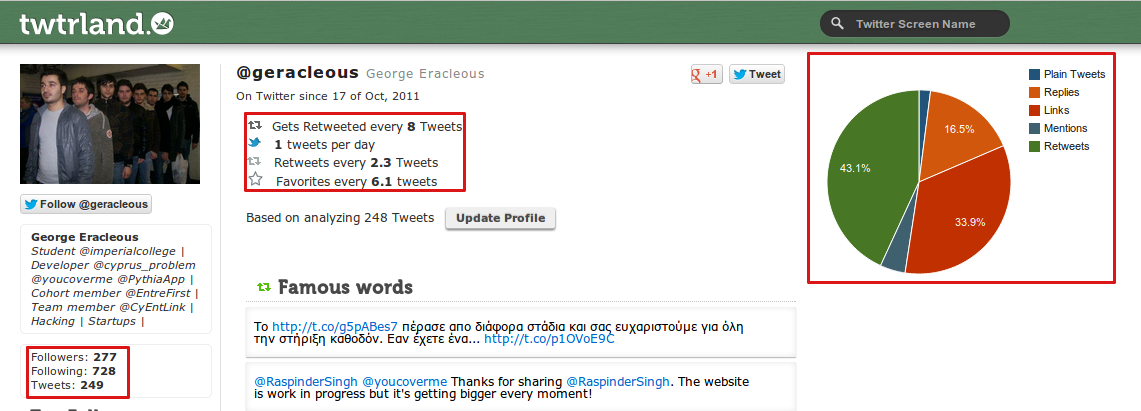
\includegraphics[height=1.9in, width=6in]{twtrland-page}
    \caption{A typical Twtrland user profile. The information in the circles is retrieved by our crawler and used in the construction of the user feature vector.}
    \label{TwtrlandPage}
  \end{center}
\end{figure} 

\subsection{Constructing the feature vectors}
Based on the information we have collected using our crawlers we can very easily construct a feature vector for each user. The vector has one column for each of the six attributes we 
defined above. Some examples of feature vectors are shown in Table \ref{FeatureVectors}. The columns represent the retweet ratio, link ratio, how often this user gets retweeted, replies ratio, mentions ratio and Followers to Followees ratio (FF) respectively. 

\begin{table}[htbp]
\footnotesize
\centering
\begin{tabular}{ l  l  l  l  l  l  l }
  \hline
  \textbf{User} & \textbf{Retweets} & \textbf{Links} & \textbf{Retweeted} & \textbf{Replies} & \textbf{Mentions} & \textbf{F/F} \\ \hline
  \emph{nytimes} & 0.0540 & 0.9091 & 0.6700 & 0.0043 & 0.0033 & 7089.2700 \\
  \emph{aplusk} & 0.0970 & 0.4042 & 0.5000 & 0.1971 & 0.0880 & 14151.1944 \\
  \emph{bencnn} & 0.2702 & 0.0974 & 0.4500 & 0.0988 & 0.0093 & 186.1068 \\
  \emph{alaa} & 0.2500 & 0.0407 & 0.8700 & 0.5120 & 0.0733 & 134.4679 \\
  \hline
\end{tabular}
\caption{The feature vectors of different types of users users}
\label{FeatureVectors}
\end{table}

The first user is the Twitter account of New York times and it is representative of the feature vectors for media organisations. Low retweet rate and a large proportion of their tweets contain links as expected. Their Followers to Followees (FF) ratio is very high and one can easily infer by their low reply and mention ratii that they almost never engage in a conversation. The second example is Ashton Kutcher, a famous Hollywood actor. His FF ratio is very high as expected and another important observation is that his replies ratio is relatively high meaning that he usually chats with other users. The username bencnn belongs Ben Wedeman a famous American journalist working for CNN. An interesting observation is that his tweets are retweeted a lot. More specifically, he gets retweeted every 0.45 tweets which is the highest rate from all four examples. This is expected as he usually tweets content that people find interesting and worth sharing. Finally, the fourth example profile belongs to Alaa Abd El-Fattah, a well known Egyptian political activist. In his profile we can observe relatively low FF ratio but very high replies ratio which is expected as he usually engages in conversations with other users.

\subsection{Software architecture}
Figure \ref{Classifiers} depicts the software architecture of the user classification module. Once again we wanted to make it as easy as possible to swap implementations of classifiers and therefore
the AbstractClassifier class factors the common functioniality of classifiers leaving the concrete implementations to the derived classes. 

\begin{figure}[htbp]
  \begin{center}
    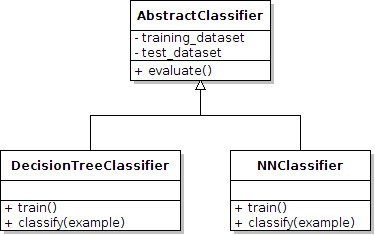
\includegraphics[height=2in, width=4in]{classifiers}
    \caption{The two derived classifiers share common functionality which is implemented in the AbstractClassifier class. }
    \label{Classifiers}
  \end{center}
\end{figure} 

\subsubsection{IDE3Classifier}
One of the most popular decision tree learning algorithms is the ID3 and there are a lot of open source implementations of it. It learns a decision trees by constructing it topdown iteratively and 
at each iteration it tries to find the best attribute from the feature vector to be tested, i.e. the attribute that helps the most in disciminating the examples). It selects this attribute using
a statistical test to determine how well it alone classifies the training examples.\\\\
We have decided to use Orange's decision tree implementation which can easily extended to incorporate new functionality. In particular, in our implementation we have written wrapper functions for training and testing a classifier around Orange's functions. We train the classifier with the labelled user examples we have collected using our crawlers and then using the learned tree it can classify unkown examples. A part of the learned tree based on our training dataset is shown in Figure \ref{Tree}. ID3 selected the root node to be the FF ratio and this is expected since this attribute is usually enough to get an indication of the type of the user. If the FF ratio for an example is lower than 143.068 then we move to the left branch otherwise to the right one. We keep moving downwards the tree until we hit a leaf node which gives the final classification for this example. For instance if an example has FF ratio higher than 143.068, it gets retwetted in less than 0.070 tweets and the proportion of links in the tweets is lower than 0.043 then the we hit the leaf node labelled with the number $0$. This number indicates that the class of this example is "Celebrity".

\begin{figure}[htbp]
  \begin{center}
    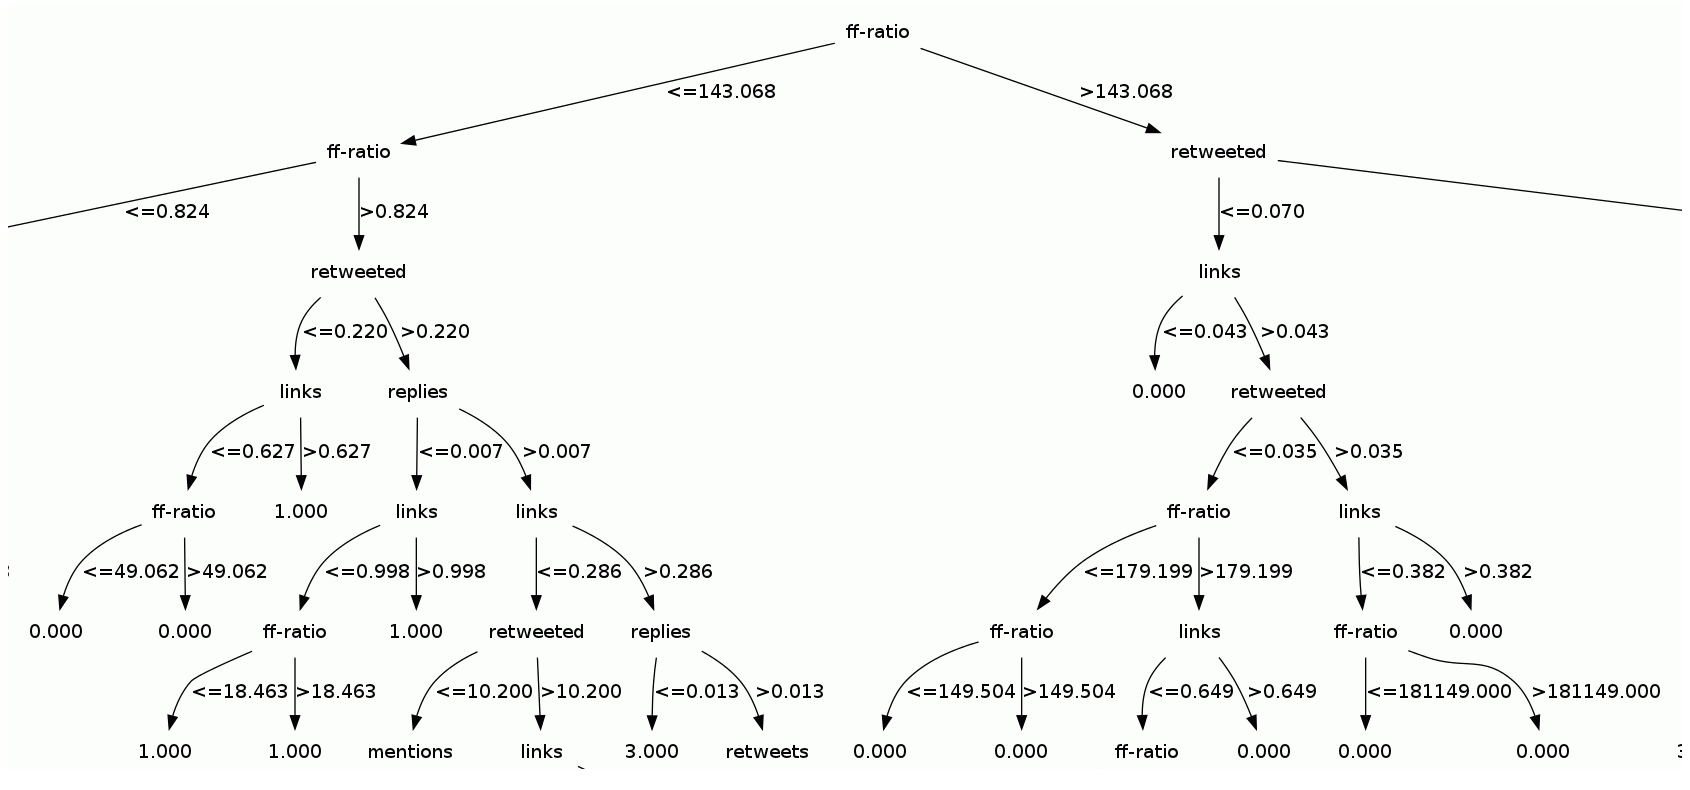
\includegraphics[height=3in, width=6in]{tree}
    \caption{Part of the decision tree learned by our classifier.}
    \label{Tree}
  \end{center}
\end{figure} 

\subsubsection{NNClassifier}


\section{Summary}

% ------------------------------------------------------------------------


%%% Local Variables: 
%%% mode: latex
%%% TeX-master: "../thesis"
%%% End: 
